% Created 2021-09-27 Mon 12:01
% Intended LaTeX compiler: xelatex
\documentclass[letterpaper]{article}
\usepackage{graphicx}
\usepackage{grffile}
\usepackage{longtable}
\usepackage{wrapfig}
\usepackage{rotating}
\usepackage[normalem]{ulem}
\usepackage{amsmath}
\usepackage{textcomp}
\usepackage{amssymb}
\usepackage{capt-of}
\usepackage{hyperref}
\setlength{\parindent}{0pt}
\usepackage[margin=1in]{geometry}
\usepackage{fontspec}
\usepackage{svg}
\usepackage{cancel}
\usepackage{indentfirst}
\setmainfont[ItalicFont = LiberationSans-Italic, BoldFont = LiberationSans-Bold, BoldItalicFont = LiberationSans-BoldItalic]{LiberationSans}
\newfontfamily\NHLight[ItalicFont = LiberationSansNarrow-Italic, BoldFont       = LiberationSansNarrow-Bold, BoldItalicFont = LiberationSansNarrow-BoldItalic]{LiberationSansNarrow}
\newcommand\textrmlf[1]{{\NHLight#1}}
\newcommand\textitlf[1]{{\NHLight\itshape#1}}
\let\textbflf\textrm
\newcommand\textulf[1]{{\NHLight\bfseries#1}}
\newcommand\textuitlf[1]{{\NHLight\bfseries\itshape#1}}
\usepackage{fancyhdr}
\pagestyle{fancy}
\usepackage{titlesec}
\usepackage{titling}
\makeatletter
\lhead{\textbf{\@title}}
\makeatother
\rhead{\textrmlf{Compiled} \today}
\lfoot{\theauthor\ \textbullet \ \textbf{2021-2022}}
\cfoot{}
\rfoot{\textrmlf{Page} \thepage}
\renewcommand{\tableofcontents}{}
\titleformat{\section} {\Large} {\textrmlf{\thesection} {|}} {0.3em} {\textbf}
\titleformat{\subsection} {\large} {\textrmlf{\thesubsection} {|}} {0.2em} {\textbf}
\titleformat{\subsubsection} {\large} {\textrmlf{\thesubsubsection} {|}} {0.1em} {\textbf}
\setlength{\parskip}{0.45em}
\renewcommand\maketitle{}
\author{Houjun Liu}
\date{\today}
\title{Viral Genetic Modulation}
\hypersetup{
 pdfauthor={Houjun Liu},
 pdftitle={Viral Genetic Modulation},
 pdfkeywords={},
 pdfsubject={},
 pdfcreator={Emacs 28.0.50 (Org mode 9.4.4)}, 
 pdflang={English}}
\begin{document}

\tableofcontents



\section{Viral Genetic Mutations}
\label{sec:orgaf0508d}
\subsection{Genetic Shift}
\label{sec:org7169f8e}
Whole segments of genome exchange abruptly as two flu viruses infect the
same cell to create a new strand. There are two mechnisms by which
happens --- ( \#ASK ) the \textbf{crossing-over mechnism} and \textbf{genome segment
reassortment}

\subsubsection{Crossing-over}
\label{sec:org318cecb}
Self-mixing of ozaki fragments during viral recombination in the
\href{KBhBIO101DNAReplication.org}{KBhBIO101DNAReplication} process
cause sudden mutations

\subsubsection{Genome Segment Reassortment}
\label{sec:org76d98cc}
Two viruses coinfect the same cell, causing cross-talk in swapping
segments

\subsection{Genetic Drift}
\label{sec:org88594b5}
This usually occurs due an error in a polymerase-driven process, where
single/groups of nucleotides flip slowly over time due to mistakes in
\href{KBhBIO101RNAReplication.org}{KBhBIO101RNAReplication}.

The former is an environment-dependent process, where the latter is able
to be modeled as it is due to predictable transcription mistake.

\noindent\rule{\textwidth}{0.5pt}

\subsection{Mutation w.r.t.}
\label{sec:org4657a1d}
\href{KBhBIO101TypesOfViruses.org}{KBhBIO101TypesOfViruses}
:CUSTOM\textsubscript{ID}: mutation-w.r.t.-filekbhbio101typesofviruses.orgkbhbio101typesofviruses
\begin{figure}[htbp]
\centering
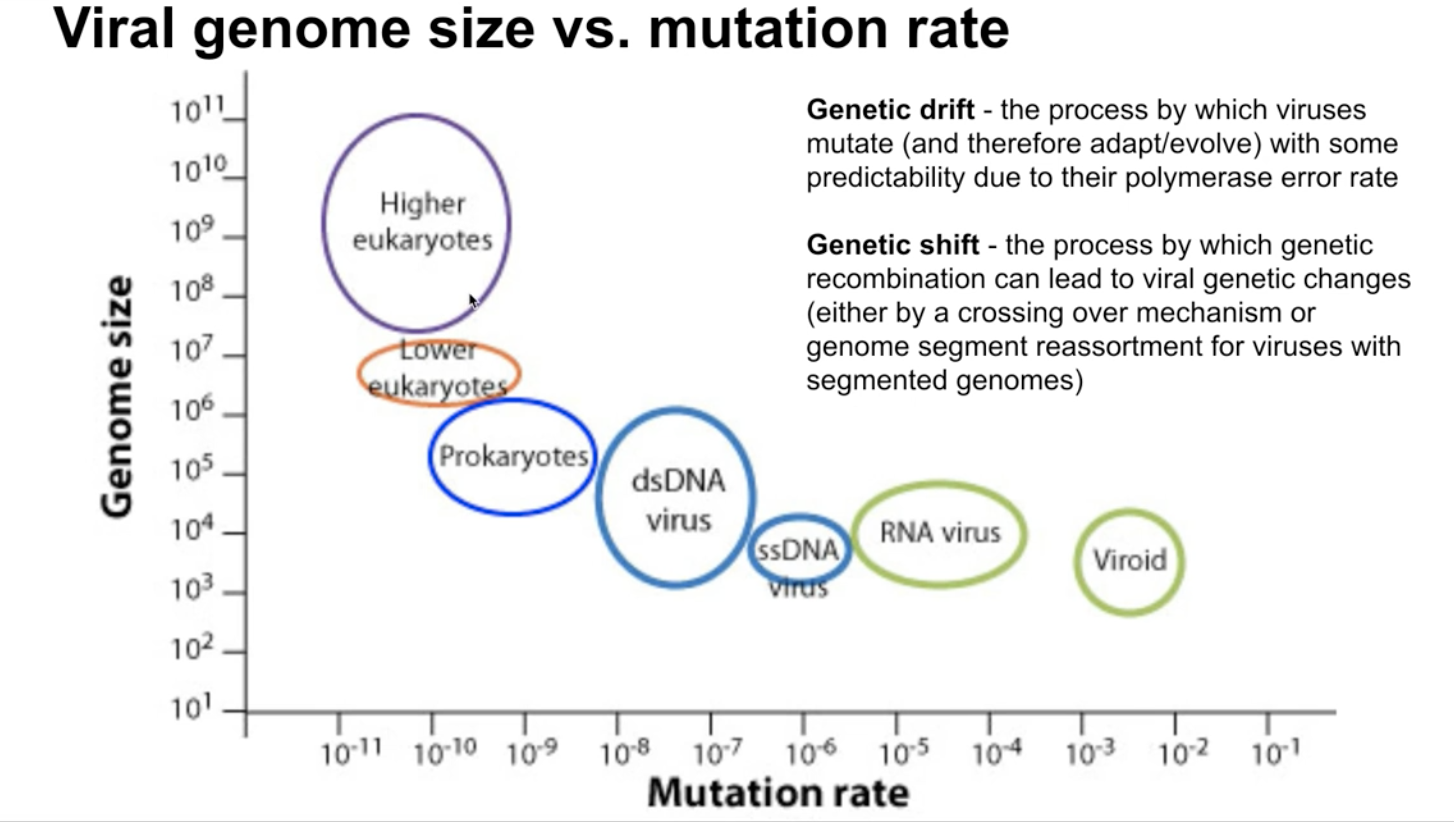
\includegraphics[width=.9\linewidth]{Screen Shot 2020-10-12 at 11.24.39 PM.png}
\caption{Screen Shot 2020-10-12 at 11.24.39 PM.png}
\end{figure}

\begin{itemize}
\item \textbf{RNA viruses} could mutate more because it does not have checks
\item \textbf{More complex+largest viruses} (DNA viruses) harder to mutate
\end{itemize}
\end{document}
